\ifdefined\beamerclass
\else
  \def\beamerclass{beamer}
\fi

\ifdefined\articlemode
  \documentclass[]{article}
  \usepackage[a4paper,margin=2cm]{geometry}
  \usepackage[envcountsect]{beamerarticle}
  \usepackage{parskip}
  \usepackage[hidelinks]{hyperref}
\else
   \documentclass[\beamerclass,ignorenonframetext]{beamer}
\fi


\usepackage{pgfpages}
\mode<handout>{
  % \setbeamercolor{background canvas}{bg=black!20}
  \pgfpagesuselayout{2 on 1}[a4paper,border shrink=5mm]
}

%\documentclass{beamer}
\mode<presentation>
{\usetheme{default}
 \usecolortheme{default}
 \usefonttheme{default}
 \setbeamertemplate{navigation symbols}{}
 \setbeamertemplate{footline}[frame number]
% \setbeamertemplate{caption}[numbered]
 }
\usepackage[english]{babel}
\usepackage{algorithm}
\usepackage[noend]{algpseudocode}
\usepackage[utf8x]{inputenc}
\usepackage{graphicx}
\usepackage{hyperref}
%\graphicspath{{./images/}}
\usepackage{tikz}
\usetikzlibrary{shapes.geometric, arrows,chains}
\usepackage{booktabs,makecell,multirow,tabularx}
\usepackage{verbatim}
\renewcommand{\arraystretch}{1.2}
\renewcommand\theadfont{\normalfont\bfseries}
\usepackage{array}
\usepackage{listings}
\lstset{language=Java, showstringspaces=false}
\usepackage[normalem]{ulem}
\usepackage{bm}
\def\layersep{2.5cm}

\usetheme{Copenhagen}
\hypersetup{pdfstartview={Fit}}
\lstset{basicstyle=\small\ttfamily,breaklines=true}

\usepackage{xcolor}
%\usepackage{subfig}
\setbeamertemplate{caption}{\insertcaption}
\usepackage[caption=false]{subfig}
\usepackage{hyperref}
\usepackage{verbatim}
%\setbeamertemplate{caption}[numbered]%\numberwithin{figure}{section}
% Define block styles
\tikzstyle{decision} = [diamond, draw, fill=blue!20, 
    text width=4.5em, text badly centered, node distance=3cm, inner sep=0pt]
\tikzstyle{block} = [rectangle, draw, fill=blue!20, 
    text width=3em, text centered, rounded corners, minimum height=3em]
\tikzstyle{line} = [draw, -latex']
\tikzstyle{cloud} = [draw, ellipse, fill=red!20, node distance=3cm,
    minimum height=2em]
\tikzset{
  startstop/.style={
    rectangle, 
    rounded corners,
    minimum width=3cm, 
    minimum height=1cm,
    align=center, 
    draw=black, 
    fill=red!30
    },
  process/.style={
    rectangle, 
    minimum width=3cm, 
    minimum height=1cm, 
    align=center, 
    draw=black, 
    fill=blue!30
    },
  decision/.style={
    rectangle, 
    minimum width=3cm, 
    minimum height=1cm, align=center, 
    draw=black, 
    fill=green!30
    },
  arrow/.style={thick,->,>=stealth},
  dec/.style={
    ellipse, 
    align=center, 
    draw=black, 
    fill=green!30
    },
}
\tikzstyle{arrow} = [thick,->,>=stealth]

\tikzset{onslide/.code args={<#1>#2}{%
  \only<#1>{\pgfkeysalso{#2}} % \pgfkeysalso doesn't change the path
}}

\makeatletter
\newenvironment<>{btHighlight}[1][]
{\begin{onlyenv}#2\begingroup\tikzset{bt@Highlight@par/.style={#1}}\begin{lrbox}{\@tempboxa}}
{\end{lrbox}\bt@HL@box[bt@Highlight@par]{\@tempboxa}\endgroup\end{onlyenv}}

\newcommand<>\btHL[1][]{%
  \only#2{\begin{btHighlight}[#1]\bgroup\aftergroup\bt@HL@endenv}%
}
\def\bt@HL@endenv{%
  \end{btHighlight}%   
  \egroup
}
\newcommand{\bt@HL@box}[2][]{%
  \tikz[#1]{%
    \pgfpathrectangle{\pgfpoint{1pt}{0pt}}{\pgfpoint{\wd #2}{\ht #2}}%
    \pgfusepath{use as bounding box}%
    \node[anchor=base west, fill=orange!30,outer sep=0pt,inner xsep=1pt, inner ysep=0pt, rounded corners=3pt, minimum height=\ht\strutbox+1pt,#1]{\raisebox{1pt}{\strut}\strut\usebox{#2}};
  }%
}
\makeatother




%%%%%%%%%%%%%%%%%%%%%%%%%%%%%%%%%%%%%%%%%%%%%%
% Formatting for title page
\title[Deep Learning]{Going Deep}
\author{Jonathon Hare}
\institute[]
{
  Vision, Learning and Control\\
  University of Southampton 
}
\date{}
\subject{Computer Science}
\useoutertheme{infolines}
\setbeamertemplate{headline}{} %remove headline
\setbeamertemplate{navigation symbols}{} %remove navigation symbols

%%%%%%%%%%%%%%%%%%%%%%%%%%%%%%%%%%%%%%%%%%%%%%

\definecolor{darkblue}{RGB}{37,55,97}
\definecolor{mellowyellow}{RGB}{247,206,70}
\definecolor{almostwhite}{RGB}{254,255,255}
\definecolor{merrygreen}{RGB}{79,173,91}
\definecolor{funkyorange}{RGB}{240,154,56}

\addtobeamertemplate{footnote}{\hskip -2em}{}
\newcommand\blfootnote[1]{%
  \begingroup
  \renewcommand\thefootnote{}\footnote{#1}%
  \addtocounter{footnote}{-1}%
  \endgroup
}

\DeclareMathOperator{\softmax}{softmax}
\DeclareMathOperator{\ReLU}{ReLU}

\begin{document}
\mode<article>{\maketitle}

\mode<presentation>{
\begin{frame}[plain]
  \begin{tikzpicture}[overlay, remember picture, shift={(current page.south west)},font={\fontfamily{Montserrat-TOsF}\selectfont}]
  \fill [funkyorange,text=darkblue] (0,0) rectangle (\paperwidth, \paperheight);
  \draw (4,7) node [align=left,text=darkblue] {\Huge \begin{tabular}{l} \textbf{Approximate} \\ \textbf{Functions} \end{tabular}};
  \draw (11,1) node [align=left,text=darkblue] {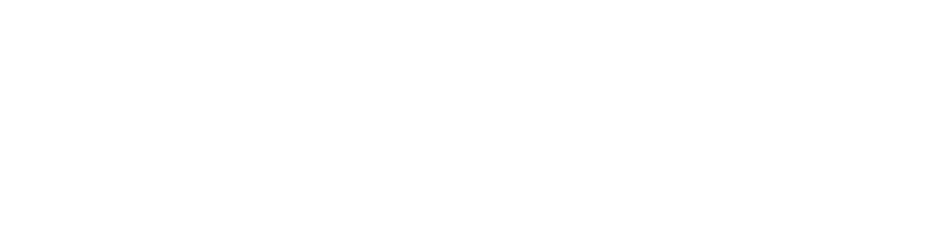
\includegraphics[scale=0.15]{../vlc.png}};
  \end{tikzpicture}
\end{frame}}


\begin{frame}
  \titlepage
\end{frame}
%-------------------------------------------------------------%
\begin{frame}\frametitle{Overview} 
\begin{itemize}
  \item No free lunch and universal approximation
  \item Why go deep?
  \item Problems of going deep
  \item Some fixes:
  \begin{itemize}
    \item Improving gradient flow with skip connections
    \item Regularising with Dropout
  \end{itemize}
\end{itemize}
\end{frame}
%-------------------------------------------------------------%
\begin{frame}\frametitle{No Free Lunch} 
\begin{itemize}
  \item<+-> Statistical learning theory claims that a machine can generalise well from a finite training set.
  \item<+-> This contradicts basic inductive reasoning which says to derive a rule describing every member of a set one must have information about every member.
  \item<+-> Machine learning avoids this problem by learning probabilistic\footnote{or perhaps more generally rules which are not certain} rules which are \emph{probably} correct about \emph{most} members of the set they concern.
  \item<+-> But, \textbf{no free lunch theorem} states that every possible classification machine has the \emph{same error} when averaged over \emph{all possible} data-generating distributions.
  \begin{itemize}
    \item<+-> \textbf{No machine learning algorithm is universally better than any other!}
    \item<+-> Fortunately, in the real world, data is generated by a small subset of generating distributions...
  \end{itemize}
\end{itemize}
\end{frame}
%-------------------------------------------------------------%

\begin{frame}{pause}\frametitle{The Universal Approximation Theorem} 
Let $\psi :\mathbb {R} \to \mathbb {R}$ be a nonconstant, bounded, and continuous function.  \pause
Let $ I_{m}$ denote the m-dimensional unit hypercube $[0,1]^m$. \pause
The space of real-valued continuous functions on $ I_{m}$ is denoted by $C(I_{m})$.  \pause 
Then, given any $\varepsilon > 0$ and any function $f \in C(I_{m})$, there exists an integer $N$, real constants $v_i, b_i \in \mathbb{R} $ and real vectors $w_{i} \in \mathbb {R} ^{m}$ for $i=1,\ldots ,N$, such that we may define: \newline

$ F(x)=\sum _{i=1}^{N}v_{i} \psi (w_{i}^{T}x+b_{i}) $
as an approximate realization of the function $f$ ; that is, \pause \newline

$|F(x)-f(x)|<\varepsilon \; \forall \; x \in I_{m}$. 
\\[1em]
\pause
$\implies$ simple neural networks can represent a wide variety of interesting functions when given appropriate parameters.
\end{frame}
%-------------------------------------------------------------%

\begin{frame}\frametitle{So a single hidden layer network can approximate most functions?} 
\begin{itemize}
\item<+-> Yes!
\item<+-> But, ...
\begin{itemize}
  \item<+-> to get the precision you require (small $\varepsilon$), you might need a really large number of hidden units (very large $N$).
  \item<+-> worse-case analysis shows it might be exponential (possibly one hidden unit for \emph{every} input configuration)
  \item<+-> We've not said anything about learnability... 
  \begin{itemize}
    \item<+-> The optimiser might not find a good solution\only<6->{\footnote{note that it has been shown that the gradients of the function are approximated by the network to an arbitrary precision}}.
    \item<+-> The training algorithm might just choose the wrong solution as a result of overfitting.
    \item<+-> \emph{There is no known universal procedure for examining a set of examples and choosing a function that will generalise to points out of the training set.}
  \end{itemize}
\end{itemize}
\end{itemize}
\end{frame}

%-------------------------------------------------------------%

\begin{frame}\frametitle{Then Why Go Deep?} 
\begin{itemize}
\item<+-> There are functions you can compute with a deep neural network that shallow networks require exponentially more hidden units to compute.
\begin{itemize}
  \item The following function is more efficient to implement using a deep neural network: $y = x_1 \oplus x_2 \oplus x_3 \oplus \dots \oplus x_n$
\end{itemize}
\item<+-> We should care about the data generating distribution (c.f. NFL). 
\begin{itemize}
  \item<+-> Real-world data has significant structure; often believed to be generated by (relatively) simple low-dimensional latent processes.
  \item<+-> Implies a prior belief that the underlying factors of variation in data can be explained by a hierarchical composition of increasingly simple latent factors 
\end{itemize}
\item<+-> Alternatively, one could just consider that a deep architecture just expresses that the function we wish to learn is a program made of multiple steps where each step makes use of the previous steps outputs.
\item<+-> \textbf{Empirically, deeper networks just seem to generalise better!}
\end{itemize}
\end{frame}
%-------------------------------------------------------------%

\begin{frame}\frametitle{What are the problems?} 
\begin{itemize}
  \item<+-> Learnability is still hard
  \begin{itemize}
    \item<+-> Problems of gradient flow
    \item<+-> Horrible symmetries in the loss landscape
    \item<+-> Overfitting
  \end{itemize}
\end{itemize}
\end{frame}

%-------------------------------------------------------------%
\begin{frame}{pause}\frametitle{Vanishing and Exploding Gradients}
\begin{itemize}
\item The vanishing and exploding gradient problem is a difficulty found in training NN with gradient-based learning methods and backpropagation.  \pause
\item In training, the gradient may become vanishingly small (or large), effectively preventing the weight from changing its value (or exploding in value). \pause
\item This leads to the neural network not being able to train. \pause
\item This issue affects many-layered networks (feed-forward), as well as recurrent networks. \pause
\item In principle, optimisers that rescale the gradients of each weight should be able to deal with this issue (as long as numeric precision doesn't become problematic).
\end{itemize}
\end{frame}
%-------------------------------------------------------------%

\begin{frame}{pause}\frametitle{Issues with Going Deep}
\centering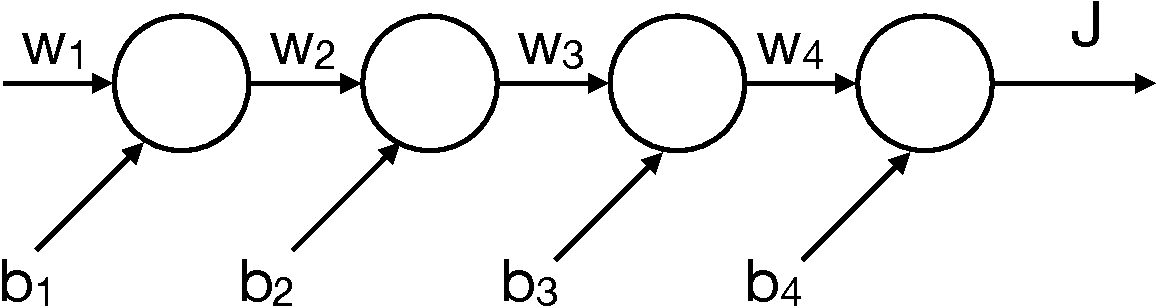
\includegraphics[width=10cm]{deep.pdf}
\end{frame}
%-------------------------------------------------------------%

\begin{frame}{pause}\frametitle{Residual Connections}

\begin{itemize}
\item One of the most effective ways to resolve diminishing gradients is with residual neural networks (ResNets)\footnote{K. He, X. Zhang, S. Ren and J. Sun, "Deep Residual Learning for Image Recognition," CVPR, Las Vegas, NV, 2016, pp. 770-778.}. \pause
\item ResNets are artificial neural networks that use {\em skip connections} to jump over  layers. \pause
\item The vanishing gradient problem is mitigated in ResNets by reusing activations from a previous layer. \pause
\item Is this the full story though? Skip connections also break symmetries, which could be much more important...
\end{itemize}
\end{frame}
%-------------------------------------------------------------%

\begin{frame}{pause}\frametitle{Residual Connections}

\centering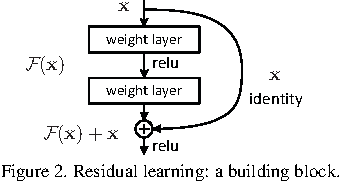
\includegraphics{ResBlock.pdf} \blfootnote{K. He, X. Zhang, S. Ren and J. Sun, "Deep Residual Learning for Image Recognition," CVPR, Las Vegas, NV, 2016, pp. 770-778.}.
\end{frame}
%-------------------------------------------------------------%

\begin{frame}{pause}\frametitle{Residual Connections}
\centering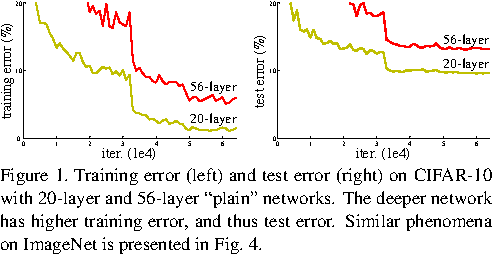
\includegraphics[width=10cm]{Fig1.pdf}\blfootnote{K. He, X. Zhang, S. Ren and J. Sun, "Deep Residual Learning for Image Recognition," CVPR, Las Vegas, NV, 2016, pp. 770-778.}
\end{frame}
%-------------------------------------------------------------%

\begin{frame}{pause}\frametitle{Residual Connections}
\centering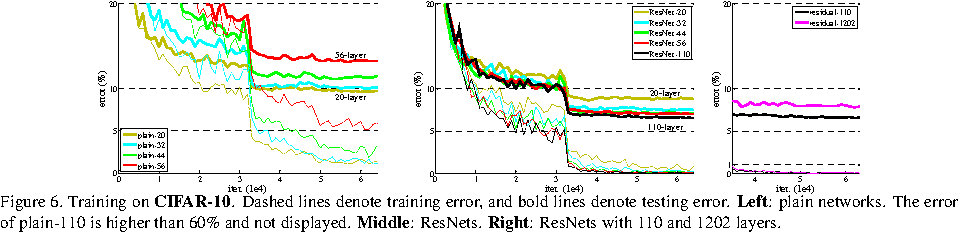
\includegraphics[width=11cm]{Fig6.pdf}\blfootnote{K. He, X. Zhang, S. Ren and J. Sun, "Deep Residual Learning for Image Recognition," CVPR, Las Vegas, NV, 2016, pp. 770-778.}
\end{frame}
%-------------------------------------------------------------%

\begin{frame}\frametitle{Overfitting}
\begin{itemize}
\item<+-> Neural networks with a large number of parameters (and hidden layers) are powerful, however, overfitting is a serious problem in such systems.
\item<+-> Just as you've seen in simple machines (e.g. Ridge Regression and LASSO), regularisation can help mitigate overfitting
\item<+-> In deep networks, we might:
\begin{itemize}
  \item<+-> Use the architecture to regularise (e.g. ConvNets)
  \item<+-> Use weight regularisers (L1, L2 [weight decay], etc, ...)
  \item<+-> Use a stochastic weight regulariser (like dropout)
  \item<+-> Regularise by smoothing the optimisation landscape (e.g. Batch Normalisation)
\end{itemize}
\end{itemize}
\end{frame}

\begin{frame}{pause}\frametitle{Dropout}
\begin{itemize}
\item Dropout is a form of regularisation \pause
\item The key idea in dropout is to randomly drop neurons, including all of the connections, from the neural network during training. \pause
\item Motivation: the best way to regularise a fixed size model is to average predictions over all possible parameter settings, weighting each setting by the posterior probability given the training data. \pause
\begin{itemize}
  \item Clearly this isn't actually tractable - dropout is an approximation of this idea.
  \item The idea of averaging predictions to resolve the bias-variance dilemma is called ensembling.
\end{itemize}
\end{itemize}
\end{frame}
%-------------------------------------------------------------%
\begin{frame}[fragile]\frametitle{Dropout}
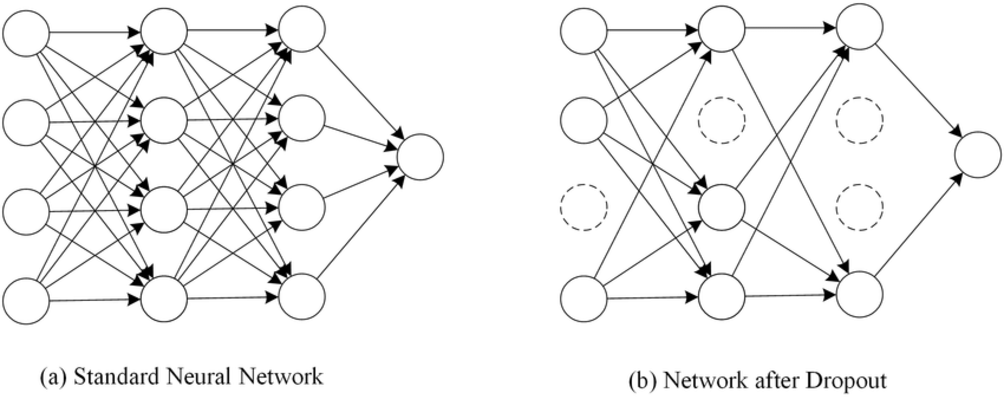
\includegraphics[width=\textwidth]{dropout.pdf} 

\blfootnote{\tiny{Image from: \url{https://www.researchgate.net/figure/Dropout-neural-network-model-a-is-a-standard-neural-network-b-is-the-same-network_fig3_309206911}}}
\end{frame}
%-------------------------------------------------------------%
\begin{frame}{pause}\frametitle{How Does Dropout Work?}
\begin{itemize}
\item In the learning phase, we set a dropout probability for each layer in the network. 
\item For each batch we then randomly decide whether or not a given neuron in a given layer is removed. \pause
\item \textbf{Inverse Dropout} scales the activations with their probability to maintain the overall magnitude of the response when dropout is disabled at evaluation/test time.
\end{itemize}
\end{frame}
%-------------------------------------------------------------%
\begin{frame}{pause}\frametitle{How is Inverted Dropout implemented?}
\begin{itemize}
\item We define a random binary mask $\bm m^{(l)}$ which is used to remove neurons and is generated by sampling a Bernoulli distribution with $P(x=1)=p$, and note, $m^{(l)}$ changes for each iteration of the backpropagation algorithm. \pause
\item The forward pass of a Dropout layer (function) during \textbf{training} is given by $f(\bm x) = \bm x \odot \bm m / p$.
\item The forward pass of a Dropout layer (function) during \textbf{inference} is given by $f(\bm x) = \bm x$. \pause
\item This can be applied to any layer(s) of the network \textit{except the output layer!} \pause
\item It's not common to put it everywhere; just a couple of select places (empirically chosen). \pause
\item The gradient (during training) is simply the hadamard product of the incoming gradient with $\bm m / p$.
% \item For layers, $l = 1$  to  $L-1$, for the forward pass of backpropagation, we then compute 
% \begin{equation}
% a^{(l)} = \sigma(w^{(l)} a^{(l - 1)} + b^{(l)})  \odot m^{(l)}
% \end{equation} \pause
% \item For layer $L$, 
% \begin{equation}
% a^{(L)} = \sigma(w^{(L)} a^{(L - 1)} + b^{(l)})
% \end{equation} \pause
% \item For the backward pass of the backpropagation algorithm, 
% \begin{equation} \delta^L = \Delta_a J \odot \sigma^{\prime} (z^L) \end{equation} \pause
% \begin{equation} \delta^l = ((w^{l + 1})^T \delta^{l + 1}) \odot \sigma^{\prime} (z^l) \odot m^{(l)} \end{equation} 
\end{itemize}
\end{frame}
%-------------------------------------------------------------%

\begin{frame}{pause}\frametitle{Why Does Dropout Work?}
\begin{itemize}
\item Neurons cannot co-adapt to other units (they cannot assume that all of the other units will be present). 
\item By breaking co-adaptation, each unit will ultimately find more general features. \pause
\item By ensembling (averaging) multiple networks, each relying on different (but overlapping) features we get a more effective machine.
\end{itemize}
\end{frame}
%-------------------------------------------------------------%
%\begin{frame}{pause}\frametitle{Batch Norm}
%\begin{itemize}
%\item Batch Normalization allows us to use much higher learning rates and be less careful about initialization.  \pause
%\item It also acts as a regularizer, in some cases eliminating the need for Dropout. 
%\end{itemize}
%\end{frame}
%-------------------------------------------------------------%

\end{document}